\documentclass{article}\usepackage[]{graphicx}\usepackage[]{xcolor}
% maxwidth is the original width if it is less than linewidth
% otherwise use linewidth (to make sure the graphics do not exceed the margin)
\makeatletter
\def\maxwidth{ %
  \ifdim\Gin@nat@width>\linewidth
    \linewidth
  \else
    \Gin@nat@width
  \fi
}
\makeatother

\definecolor{fgcolor}{rgb}{0.345, 0.345, 0.345}
\newcommand{\hlnum}[1]{\textcolor[rgb]{0.686,0.059,0.569}{#1}}%
\newcommand{\hlsng}[1]{\textcolor[rgb]{0.192,0.494,0.8}{#1}}%
\newcommand{\hlcom}[1]{\textcolor[rgb]{0.678,0.584,0.686}{\textit{#1}}}%
\newcommand{\hlopt}[1]{\textcolor[rgb]{0,0,0}{#1}}%
\newcommand{\hldef}[1]{\textcolor[rgb]{0.345,0.345,0.345}{#1}}%
\newcommand{\hlkwa}[1]{\textcolor[rgb]{0.161,0.373,0.58}{\textbf{#1}}}%
\newcommand{\hlkwb}[1]{\textcolor[rgb]{0.69,0.353,0.396}{#1}}%
\newcommand{\hlkwc}[1]{\textcolor[rgb]{0.333,0.667,0.333}{#1}}%
\newcommand{\hlkwd}[1]{\textcolor[rgb]{0.737,0.353,0.396}{\textbf{#1}}}%
\let\hlipl\hlkwb

\usepackage{framed}
\makeatletter
\newenvironment{kframe}{%
 \def\at@end@of@kframe{}%
 \ifinner\ifhmode%
  \def\at@end@of@kframe{\end{minipage}}%
  \begin{minipage}{\columnwidth}%
 \fi\fi%
 \def\FrameCommand##1{\hskip\@totalleftmargin \hskip-\fboxsep
 \colorbox{shadecolor}{##1}\hskip-\fboxsep
     % There is no \\@totalrightmargin, so:
     \hskip-\linewidth \hskip-\@totalleftmargin \hskip\columnwidth}%
 \MakeFramed {\advance\hsize-\width
   \@totalleftmargin\z@ \linewidth\hsize
   \@setminipage}}%
 {\par\unskip\endMakeFramed%
 \at@end@of@kframe}
\makeatother

\definecolor{shadecolor}{rgb}{.97, .97, .97}
\definecolor{messagecolor}{rgb}{0, 0, 0}
\definecolor{warningcolor}{rgb}{1, 0, 1}
\definecolor{errorcolor}{rgb}{1, 0, 0}
\newenvironment{knitrout}{}{} % an empty environment to be redefined in TeX

\usepackage{alltt}
\usepackage[margin=1.0in]{geometry} % To set margins
\usepackage{amsmath}  % This allows me to use the align functionality.
                      % If you find yourself trying to replicate
                      % something you found online, ensure you're
                      % loading the necessary packages!
\usepackage{amsfonts} % Math font
\usepackage{fancyvrb}
\usepackage{hyperref} % For including hyperlinks
\usepackage[shortlabels]{enumitem}% For enumerated lists with labels specified
                                  % We had to run tlmgr_install("enumitem") in R
\usepackage{float}    % For telling R where to put a table/figure
\usepackage{natbib}        %For the bibliography
\bibliographystyle{apalike}%For the bibliography
\IfFileExists{upquote.sty}{\usepackage{upquote}}{}
\begin{document}


\cite{Kasdin25} show that dopamine in the brains of young zebra finches acts as 
a learning signal, increasing when they sing closer to their adult song and 
decreasing when they sing further away, effectively guiding their vocal 
development through trial-and-error. This suggests that complex natural 
behaviors, like learning to sing, are shaped by dopamine-driven reinforcement 
learning, similar to how artificial intelligence learns. You can find the 
paper at this link:
\href{https://www.nature.com/articles/s41586-025-08729-1}{{https://www.nature.com/articles/s41586-025-08729-1}.}.

Note they measure dopamine using fibre photometry, changes in the fluorescence
indicate dopamine changes in realtime. Their specific measurement considers 
changes in flourescence in 100-ms windows between 200 and 300 ms from the start 
of singing, averaged across development.

\begin{enumerate}
%%%%%%%%%%%%%%%%%%%%%%%%%%%%%%%%%%%%%%%%%%%%%%%%%%%%%%%%%%%%%%%%%
% CONDUCT A POWER ANALYSIS
%%%%%%%%%%%%%%%%%%%%%%%%%%%%%%%%%%%%%%%%%%%%%%%%%%%%%%%%%%%%%%%%%
\item Using the \texttt{pwr} package for \texttt{R} \citep{pwr},
conduct a power analysis. How many observations would the researchers 
need to detect a moderate-to-large effect ($d=0.65$) when using 
$\alpha=0.05$ and default power (0.80) for a two-sided one sample 
$t$ test?

\begin{knitrout}\scriptsize
\definecolor{shadecolor}{rgb}{0.969, 0.969, 0.969}\color{fgcolor}\begin{kframe}
\begin{alltt}
\hlkwd{library}\hldef{(pwr)}
\hlkwd{set.seed}\hldef{(}\hlnum{5656}\hldef{)}

\hldef{(}\hlkwd{pwr.t.test}\hldef{(}\hlkwc{d} \hldef{=} \hlnum{0.65}\hldef{,}
           \hlkwc{power} \hldef{=} \hlnum{0.80}\hldef{,}
           \hlkwc{sig.level} \hldef{=} \hlnum{0.05}\hldef{,}
           \hlkwc{alternative} \hldef{=} \hlsng{"two.sided"}\hldef{,}
           \hlkwc{type} \hldef{=} \hlsng{"one.sample"}\hldef{))}
\end{alltt}
\begin{verbatim}
## 
##      One-sample t test power calculation 
## 
##               n = 20.58039
##               d = 0.65
##       sig.level = 0.05
##           power = 0.8
##     alternative = two.sided
\end{verbatim}
\end{kframe}
\end{knitrout}

Since $n = 20.58039$, at least 21 observations are needed to detect a moderate-to-large effect.

%%%%%%%%%%%%%%%%%%%%%%%%%%%%%%%%%%%%%%%%%%%%%%%%%%%%%%%%%%%%%%%%%
% COLLECT DATA
%%%%%%%%%%%%%%%%%%%%%%%%%%%%%%%%%%%%%%%%%%%%%%%%%%%%%%%%%%%%%%%%%
\item Click the link to go to the paper. Find the source data for 
Figure 2. Download the Excel file. Describe what you needed to
do to collect the data for Figure 2(g). Note that you only need the 
\texttt{closer\_vals} and \texttt{further\_vals}. Ensure to 
\texttt{mutate()} the data to get a difference 
(e.g., \texttt{closer\_vals - further\_vals}).

\begin{knitrout}\scriptsize
\definecolor{shadecolor}{rgb}{0.969, 0.969, 0.969}\color{fgcolor}\begin{kframe}
\begin{alltt}
\hlkwd{library}\hldef{(tidyverse)}

\hldef{farther} \hlkwb{<-} \hlkwd{read_csv}\hldef{(}\hlsng{"farther.csv"}\hldef{,}\hlkwc{col_names} \hldef{= F)}
\hldef{closer} \hlkwb{<-} \hlkwd{read_csv}\hldef{(}\hlsng{"closer.csv"}\hldef{,}\hlkwc{col_names} \hldef{= F)}

\hldef{fig.2g.data} \hlkwb{<-} \hlkwd{tibble}\hldef{(}\hlkwc{g.Farther_vals} \hldef{= farther[[}\hlnum{1}\hldef{]],}
                      \hlkwc{g.Closer_vals} \hldef{= closer[[}\hlnum{1}\hldef{]]) |>}
  \hlkwd{mutate}\hldef{(}\hlkwc{difference} \hldef{= g.Closer_vals} \hlopt{-} \hldef{g.Farther_vals)}
\hlcom{#view(fig.2g.data)}
\end{alltt}
\end{kframe}
\end{knitrout}

To collect the data for Figure 2(g), the g.Farther\_vals and g.Closer\_vals columns were downloaded, converted to csv files, and merged into a tibble. Their difference was then calculated and mutated as a third column.

%%%%%%%%%%%%%%%%%%%%%%%%%%%%%%%%%%%%%%%%%%%%%%%%%%%%%%%%%%%%%%%%%
% SUMMARIZE DATA
%%%%%%%%%%%%%%%%%%%%%%%%%%%%%%%%%%%%%%%%%%%%%%%%%%%%%%%%%%%%%%%%%
\item Summarize the data.
\begin{enumerate}
  \item Summarize the further data. Do the data suggest that
   dopamine in the brains of young zebra finches decreases when
   they sing further away?

\begin{knitrout}\scriptsize
\definecolor{shadecolor}{rgb}{0.969, 0.969, 0.969}\color{fgcolor}\begin{kframe}
\begin{alltt}
\hlkwd{library}\hldef{(e1071)}

\hldef{farther.summary} \hlkwb{<-} \hldef{fig.2g.data |>}
  \hlkwd{summarize}\hldef{(}\hlkwc{mean}       \hldef{=} \hlkwd{mean}\hldef{(g.Farther_vals),}
            \hlkwc{sd}         \hldef{=} \hlkwd{sd}\hldef{(g.Farther_vals),}
            \hlkwc{median}     \hldef{=} \hlkwd{median}\hldef{(g.Farther_vals),}
            \hlkwc{IQR}        \hldef{=} \hlkwd{IQR}\hldef{(g.Farther_vals),}
            \hlkwc{skewness}   \hldef{=} \hlkwd{skewness}\hldef{(g.Farther_vals),}
            \hlkwc{exkurtosis} \hldef{=} \hlkwd{kurtosis}\hldef{(g.Farther_vals))}

\hldef{(farther.summary)}
\end{alltt}
\begin{verbatim}
## # A tibble: 1 x 6
##     mean    sd median   IQR skewness exkurtosis
##    <dbl> <dbl>  <dbl> <dbl>    <dbl>      <dbl>
## 1 -0.203 0.130 -0.187 0.187    -1.04       1.19
\end{verbatim}
\end{kframe}
\end{knitrout}
Since the mean is less than zero, the data suggest that on average, dopamine in the brains of young zebra finches decreases when they sing further away.

   \item Summarize the closer data. Do the data suggest that
   dopamine in the brains of young zebra finches increases when
   they sing closer to their adult song?

\begin{knitrout}\scriptsize
\definecolor{shadecolor}{rgb}{0.969, 0.969, 0.969}\color{fgcolor}\begin{kframe}
\begin{alltt}
\hldef{closer.summary} \hlkwb{<-} \hldef{fig.2g.data |>}
  \hlkwd{summarize}\hldef{(}\hlkwc{mean}       \hldef{=} \hlkwd{mean}\hldef{(g.Closer_vals),}
            \hlkwc{sd}         \hldef{=} \hlkwd{sd}\hldef{(g.Closer_vals),}
            \hlkwc{median}     \hldef{=} \hlkwd{median}\hldef{(g.Closer_vals),}
            \hlkwc{IQR}        \hldef{=} \hlkwd{IQR}\hldef{(g.Closer_vals),}
            \hlkwc{skewness}   \hldef{=} \hlkwd{skewness}\hldef{(g.Closer_vals),}
            \hlkwc{exkurtosis} \hldef{=} \hlkwd{kurtosis}\hldef{(g.Closer_vals))}

\hldef{(closer.summary)}
\end{alltt}
\begin{verbatim}
## # A tibble: 1 x 6
##    mean     sd median   IQR skewness exkurtosis
##   <dbl>  <dbl>  <dbl> <dbl>    <dbl>      <dbl>
## 1 0.156 0.0941  0.146 0.107    0.295     -0.859
\end{verbatim}
\end{kframe}
\end{knitrout}
Since the mean is greater than zero, the data suggest that on average, dopamine in the brains of young zebra finches increases when they sing closer to their adult song.

  \item Summarize the paired differences. Do the data suggest
  that there is a difference between dopamine in the brains of
  young zebra finches when they sing further away compared to 
  closer to their adult song?

\begin{knitrout}\scriptsize
\definecolor{shadecolor}{rgb}{0.969, 0.969, 0.969}\color{fgcolor}\begin{kframe}
\begin{alltt}
\hldef{difference.summary} \hlkwb{<-} \hldef{fig.2g.data |>}
  \hlkwd{summarize}\hldef{(}\hlkwc{mean}       \hldef{=} \hlkwd{mean}\hldef{(difference),}
            \hlkwc{sd}         \hldef{=} \hlkwd{sd}\hldef{(difference),}
            \hlkwc{median}     \hldef{=} \hlkwd{median}\hldef{(difference),}
            \hlkwc{IQR}        \hldef{=} \hlkwd{IQR}\hldef{(difference),}
            \hlkwc{skewness}   \hldef{=} \hlkwd{skewness}\hldef{(difference),}
            \hlkwc{exkurtosis} \hldef{=} \hlkwd{kurtosis}\hldef{(difference))}

\hldef{(difference.summary)}
\end{alltt}
\begin{verbatim}
## # A tibble: 1 x 6
##    mean    sd median   IQR skewness exkurtosis
##   <dbl> <dbl>  <dbl> <dbl>    <dbl>      <dbl>
## 1 0.359 0.211  0.332 0.239    0.773      0.128
\end{verbatim}
\end{kframe}
\end{knitrout}
Since the mean is significantly far from zero, it appears that there is a distinct difference between dopamine in the brains of
young zebra finches when they sing further away compared to 
closer to their adult song.

  \item \textbf{Optional Challenge:} Can you reproduce Figure 2(g)?
  Note that the you can use \texttt{geom\_errorbar()} to plot
  the range created by adding the mean $\pm$ one standard deviation.
\end{enumerate}
%%%%%%%%%%%%%%%%%%%%%%%%%%%%%%%%%%%%%%%%%%%%%%%%%%%%%%%%%%%%%%%%%
% CONDUCT THE TESTS
%%%%%%%%%%%%%%%%%%%%%%%%%%%%%%%%%%%%%%%%%%%%%%%%%%%%%%%%%%%%%%%%%
\item Conduct the inferences they do in the paper. Make sure to report the results
a little more comprehensively -- that is your parenthetical should look something
like: ($t=23.99$, $p<0.0001$; $g=1.34$; 95\% CI: 4.43, 4.60).\\
\textbf{Note:} Your numbers may vary slightly as they performed some unclear
correction of their $p$-values. I'm waiting to hear back from them via email!
\begin{enumerate}
  \item ``The close responses differed significantly from 0 ($p=1.63 \times 10^{-8}$).''
  
\begin{knitrout}\scriptsize
\definecolor{shadecolor}{rgb}{0.969, 0.969, 0.969}\color{fgcolor}\begin{kframe}
\begin{alltt}
\hlkwd{library}\hldef{(effectsize)}

\hlcom{# a) Closer}

\hldef{mu0} \hlkwb{<-} \hlnum{0}
\hldef{x} \hlkwb{<-} \hldef{fig.2g.data}\hlopt{$}\hldef{g.Closer_vals}
\hldef{xbar} \hlkwb{<-} \hlkwd{mean}\hldef{(x)}
\hldef{s} \hlkwb{<-} \hlkwd{sd}\hldef{(x)}
\hldef{n} \hlkwb{<-} \hlkwd{length}\hldef{(x)}
\hldef{(t.stat.a} \hlkwb{<-} \hldef{(xbar} \hlopt{-} \hldef{mu0)}\hlopt{/}\hldef{(s}\hlopt{/}\hlkwd{sqrt}\hldef{(n)))}
\end{alltt}
\begin{verbatim}
## [1] 8.302409
\end{verbatim}
\begin{alltt}
\hldef{(p.val} \hlkwb{<-} \hlnum{2}\hlopt{*}\hlkwd{pt}\hldef{(}\hlkwc{q}\hldef{=}\hlopt{-}\hlkwd{abs}\hldef{(t.stat.a),} \hlkwc{df} \hldef{= n}\hlopt{-}\hlnum{1}\hldef{))}
\end{alltt}
\begin{verbatim}
## [1] 1.626307e-08
\end{verbatim}
\begin{alltt}
\hlkwd{t.test}\hldef{(}\hlkwc{x}\hldef{=x,} \hlkwc{mu} \hldef{= mu0,} \hlkwc{alternative} \hldef{=} \hlsng{"greater"}\hldef{)}
\end{alltt}
\begin{verbatim}
## 
## 	One Sample t-test
## 
## data:  x
## t = 8.3024, df = 24, p-value = 8.132e-09
## alternative hypothesis: true mean is greater than 0
## 95 percent confidence interval:
##  0.1240301       Inf
## sample estimates:
## mean of x 
## 0.1562231
\end{verbatim}
\begin{alltt}
\hldef{(}\hlkwd{hedges_g}\hldef{(}\hlkwc{x} \hldef{= x,} \hlkwc{mu} \hldef{= mu0,} \hlkwc{alternative} \hldef{=} \hlsng{"greater"}\hldef{))}
\end{alltt}
\begin{verbatim}
## Hedges' g |      95% CI
## -----------------------
## 1.61      | [1.10, Inf]
## 
## - One-sided CIs: upper bound fixed at [Inf].
\end{verbatim}
\begin{alltt}
\hlkwd{interpret_hedges_g}\hldef{(}\hlnum{1.61}\hldef{)}
\end{alltt}
\begin{verbatim}
## [1] "large"
## (Rules: cohen1988)
\end{verbatim}
\begin{alltt}
\hlkwd{t.test}\hldef{(}\hlkwc{x}\hldef{=x,} \hlkwc{mu} \hldef{= mu0,} \hlkwc{alternative} \hldef{=} \hlsng{"two.sided"}\hldef{)}
\end{alltt}
\begin{verbatim}
## 
## 	One Sample t-test
## 
## data:  x
## t = 8.3024, df = 24, p-value = 1.626e-08
## alternative hypothesis: true mean is not equal to 0
## 95 percent confidence interval:
##  0.1173875 0.1950586
## sample estimates:
## mean of x 
## 0.1562231
\end{verbatim}
\end{kframe}
\end{knitrout}

The close responses differed significantly from 0 ($t=8.3024$, $p=1.626 \times 10^{-08}$; $g=1.61$; 95\% CI: 0.1173875, 0.1950586).

  \item ``The far responses differed significantly from 0 ($p=5.17 \times 10^{-8}$).''
  
\begin{knitrout}\scriptsize
\definecolor{shadecolor}{rgb}{0.969, 0.969, 0.969}\color{fgcolor}\begin{kframe}
\begin{alltt}
\hlcom{# b) Farther}

\hldef{mu0} \hlkwb{<-} \hlnum{0}
\hldef{x} \hlkwb{<-} \hldef{fig.2g.data}\hlopt{$}\hldef{g.Farther_vals}
\hldef{xbar} \hlkwb{<-} \hlkwd{mean}\hldef{(x)}
\hldef{s} \hlkwb{<-} \hlkwd{sd}\hldef{(x)}
\hldef{n} \hlkwb{<-} \hlkwd{length}\hldef{(x)}
\hldef{(t.stat.b} \hlkwb{<-} \hldef{(xbar} \hlopt{-} \hldef{mu0)}\hlopt{/}\hldef{(s}\hlopt{/}\hlkwd{sqrt}\hldef{(n)))}
\end{alltt}
\begin{verbatim}
## [1] -7.777991
\end{verbatim}
\begin{alltt}
\hldef{(p.val} \hlkwb{<-} \hlnum{2}\hlopt{*}\hlkwd{pt}\hldef{(}\hlkwc{q}\hldef{=}\hlopt{-}\hlkwd{abs}\hldef{(t.stat.b),} \hlkwc{df} \hldef{= n}\hlopt{-}\hlnum{1}\hldef{))}
\end{alltt}
\begin{verbatim}
## [1] 5.174718e-08
\end{verbatim}
\begin{alltt}
\hlkwd{t.test}\hldef{(}\hlkwc{x}\hldef{=x,} \hlkwc{mu} \hldef{= mu0,} \hlkwc{alternative} \hldef{=} \hlsng{"less"}\hldef{)}
\end{alltt}
\begin{verbatim}
## 
## 	One Sample t-test
## 
## data:  x
## t = -7.778, df = 24, p-value = 2.587e-08
## alternative hypothesis: true mean is less than 0
## 95 percent confidence interval:
##        -Inf -0.1581322
## sample estimates:
##  mean of x 
## -0.2027244
\end{verbatim}
\begin{alltt}
\hldef{(}\hlkwd{hedges_g}\hldef{(}\hlkwc{x} \hldef{= x,} \hlkwc{mu} \hldef{= mu0,} \hlkwc{alternative} \hldef{=} \hlsng{"less"}\hldef{))}
\end{alltt}
\begin{verbatim}
## Hedges' g |        95% CI
## -------------------------
## -1.51     | [-Inf, -1.02]
## 
## - One-sided CIs: lower bound fixed at [-Inf].
\end{verbatim}
\begin{alltt}
\hlkwd{interpret_hedges_g}\hldef{(}\hlopt{-}\hlnum{1.51}\hldef{)}
\end{alltt}
\begin{verbatim}
## [1] "large"
## (Rules: cohen1988)
\end{verbatim}
\begin{alltt}
\hlkwd{t.test}\hldef{(}\hlkwc{x}\hldef{=x,} \hlkwc{mu} \hldef{= mu0,} \hlkwc{alternative} \hldef{=} \hlsng{"two.sided"}\hldef{)}
\end{alltt}
\begin{verbatim}
## 
## 	One Sample t-test
## 
## data:  x
## t = -7.778, df = 24, p-value = 5.175e-08
## alternative hypothesis: true mean is not equal to 0
## 95 percent confidence interval:
##  -0.2565176 -0.1489313
## sample estimates:
##  mean of x 
## -0.2027244
\end{verbatim}
\end{kframe}
\end{knitrout}
The far responses differed significantly from 0 ($t=-7.778$, $p=5.175 \times 10^{-08}$; $g=-1.51$; 95\% CI: -0.2565176, -0.1489313).

  \item ``The difference between populations was significant ($p=1.04 \times10^{-8}$).''
\begin{knitrout}\scriptsize
\definecolor{shadecolor}{rgb}{0.969, 0.969, 0.969}\color{fgcolor}\begin{kframe}
\begin{alltt}
\hlcom{# c) Difference}

\hldef{mu0} \hlkwb{<-} \hlnum{0}
\hldef{x} \hlkwb{<-} \hldef{fig.2g.data}\hlopt{$}\hldef{difference}
\hldef{xbar} \hlkwb{<-} \hlkwd{mean}\hldef{(x)}
\hldef{s} \hlkwb{<-} \hlkwd{sd}\hldef{(x)}
\hldef{n} \hlkwb{<-} \hlkwd{length}\hldef{(x)}
\hldef{(t.stat.c} \hlkwb{<-} \hldef{(xbar} \hlopt{-} \hldef{mu0)}\hlopt{/}\hldef{(s}\hlopt{/}\hlkwd{sqrt}\hldef{(n)))}
\end{alltt}
\begin{verbatim}
## [1] 8.510932
\end{verbatim}
\begin{alltt}
\hldef{(p.val} \hlkwb{<-} \hlnum{2}\hlopt{*}\hlkwd{pt}\hldef{(}\hlkwc{q}\hldef{=}\hlopt{-}\hlkwd{abs}\hldef{(t.stat.c),} \hlkwc{df} \hldef{= n}\hlopt{-}\hlnum{1}\hldef{))}
\end{alltt}
\begin{verbatim}
## [1] 1.036907e-08
\end{verbatim}
\begin{alltt}
\hlkwd{t.test}\hldef{(}\hlkwc{x}\hldef{=x,} \hlkwc{mu} \hldef{= mu0,} \hlkwc{alternative} \hldef{=} \hlsng{"two.sided"}\hldef{)}
\end{alltt}
\begin{verbatim}
## 
## 	One Sample t-test
## 
## data:  x
## t = 8.5109, df = 24, p-value = 1.037e-08
## alternative hypothesis: true mean is not equal to 0
## 95 percent confidence interval:
##  0.2719028 0.4459921
## sample estimates:
## mean of x 
## 0.3589475
\end{verbatim}
\begin{alltt}
\hldef{(}\hlkwd{hedges_g}\hldef{(}\hlkwc{x} \hldef{= x,} \hlkwc{mu} \hldef{= mu0,} \hlkwc{alternative} \hldef{=} \hlsng{"two.sided"}\hldef{))}
\end{alltt}
\begin{verbatim}
## Hedges' g |       95% CI
## ------------------------
## 1.65      | [1.04, 2.24]
\end{verbatim}
\begin{alltt}
\hlkwd{interpret_hedges_g}\hldef{(}\hlnum{1.65}\hldef{)}
\end{alltt}
\begin{verbatim}
## [1] "large"
## (Rules: cohen1988)
\end{verbatim}
\end{kframe}
\end{knitrout}
The difference between populations was significant ($t=8.5109$, $p=1.037 \times 10^{-08}$; $g=1.65$; 95\% CI: 0.2719028 0.4459921).

\end{enumerate}
%%%%%%%%%%%%%%%%%%%%%%%%%%%%%%%%%%%%%%%%%%%%%%%%%%%%%%%%%%%%%%%%%
% CONDUCT THE TESTS
%%%%%%%%%%%%%%%%%%%%%%%%%%%%%%%%%%%%%%%%%%%%%%%%%%%%%%%%%%%%%%%%%
\item Reverse engineer the hypothesis test plot from Lecture 20 to create accurate
hypothesis testing plots for each part of the previous question.
\begin{enumerate}
  \item Question 4, part(a).
\begin{knitrout}\scriptsize
\definecolor{shadecolor}{rgb}{0.969, 0.969, 0.969}\color{fgcolor}\begin{kframe}
\begin{alltt}
\hlcom{# a) Closer}

\hldef{mu0} \hlkwb{<-} \hlnum{0}
\hldef{x} \hlkwb{<-} \hldef{fig.2g.data}\hlopt{$}\hldef{g.Closer_vals}
\hldef{xbar} \hlkwb{<-} \hlkwd{mean}\hldef{(x)}
\hldef{s} \hlkwb{<-} \hlkwd{sd}\hldef{(x)}
\hldef{n} \hlkwb{<-} \hlkwd{length}\hldef{(x)}

\hldef{ggdat.t} \hlkwb{<-} \hlkwd{tibble}\hldef{(}\hlkwc{t}\hldef{=}\hlkwd{seq}\hldef{(}\hlopt{-}\hlnum{5}\hldef{,}\hlnum{5}\hldef{,}\hlkwc{length.out}\hldef{=}\hlnum{1000}\hldef{))|>}
  \hlkwd{mutate}\hldef{(}\hlkwc{pdf.null} \hldef{=} \hlkwd{dt}\hldef{(t,} \hlkwc{df}\hldef{=n}\hlopt{-}\hlnum{1}\hldef{))}
\hlcom{# For plotting the observed point}
\hldef{ggdat.obs} \hlkwb{<-} \hlkwd{tibble}\hldef{(}\hlkwc{t} \hldef{= t.stat.a,}
                    \hlkwc{y} \hldef{=} \hlnum{0}\hldef{)} \hlcom{# to plot on x-axis}

\hlcom{# Resampling to approximate the sampling distribution }
\hlcom{# on the data}
\hldef{R} \hlkwb{<-} \hlnum{1000}
\hldef{resamples} \hlkwb{<-} \hlkwd{tibble}\hldef{(}\hlkwc{t}\hldef{=}\hlkwd{numeric}\hldef{(R))}
\hlkwa{for}\hldef{(i} \hlkwa{in} \hlnum{1}\hlopt{:}\hldef{R)\{}
  \hldef{curr.sample} \hlkwb{<-} \hlkwd{sample}\hldef{(}\hlkwc{x}\hldef{=x,}
                        \hlkwc{size}\hldef{=n,}
                        \hlkwc{replace}\hldef{=T)}
  \hldef{resamples}\hlopt{$}\hldef{t[i]} \hlkwb{=} \hldef{(}\hlkwd{mean}\hldef{(curr.sample)}\hlopt{-}\hldef{mu0)}\hlopt{/}\hldef{(}\hlkwd{sd}\hldef{(curr.sample)}\hlopt{/}\hlkwd{sqrt}\hldef{(n))}
\hldef{\}}

\hldef{t.breaks} \hlkwb{<-} \hlkwd{c}\hldef{(}\hlopt{-}\hlnum{5}\hldef{,} \hlnum{0}\hldef{,}
              \hlkwd{qt}\hldef{(}\hlnum{0.95}\hldef{,} \hlkwc{df} \hldef{= n}\hlopt{-}\hlnum{1}\hldef{),} \hlnum{14}\hldef{,}  \hlcom{# rejection region (right)}
              \hldef{t.stat.a)}                  \hlcom{# t-statistic observed}
\hldef{xbar.breaks} \hlkwb{<-} \hldef{t.breaks} \hlopt{*} \hldef{s}\hlopt{/}\hldef{(}\hlkwd{sqrt}\hldef{(n))} \hlopt{+} \hldef{mu0}

\hlcom{# Create Plot}
\hlkwd{ggplot}\hldef{()} \hlopt{+}
  \hlcom{# null distribution}
  \hlkwd{geom_line}\hldef{(}\hlkwc{data}\hldef{=ggdat.t,}
            \hlkwd{aes}\hldef{(}\hlkwc{x}\hldef{=t,} \hlkwc{y}\hldef{=pdf.null))}\hlopt{+}
  \hlkwd{geom_hline}\hldef{(}\hlkwc{yintercept}\hldef{=}\hlnum{0}\hldef{)}\hlopt{+}
  \hlcom{# rejection region}
  \hlkwd{geom_ribbon}\hldef{(}\hlkwc{data}\hldef{=}\hlkwd{subset}\hldef{(ggdat.t, t}\hlopt{>=}\hlkwd{qt}\hldef{(}\hlnum{0.95}\hldef{,} \hlkwc{df}\hldef{=n}\hlopt{-}\hlnum{1}\hldef{)),}
              \hlkwd{aes}\hldef{(}\hlkwc{x}\hldef{=t,} \hlkwc{ymin}\hldef{=}\hlnum{0}\hldef{,} \hlkwc{ymax}\hldef{=pdf.null),}
              \hlkwc{fill}\hldef{=}\hlsng{"grey"}\hldef{,} \hlkwc{alpha}\hldef{=}\hlnum{0.5}\hldef{)}\hlopt{+}
  \hlcom{# plot p-value (not visible)}
  \hlkwd{geom_ribbon}\hldef{(}\hlkwc{data}\hldef{=}\hlkwd{subset}\hldef{(ggdat.t, t}\hlopt{>=}\hldef{t.stat.a),}
              \hlkwd{aes}\hldef{(}\hlkwc{x}\hldef{=t,} \hlkwc{ymin}\hldef{=}\hlnum{0}\hldef{,} \hlkwc{ymax}\hldef{=pdf.null),}
              \hlkwc{fill}\hldef{=}\hlsng{"white"}\hldef{,} \hlkwc{alpha}\hldef{=}\hlnum{0.25}\hldef{)}\hlopt{+}
  \hlcom{# plot observation point}
  \hlkwd{geom_point}\hldef{(}\hlkwc{data}\hldef{=ggdat.obs,} \hlkwd{aes}\hldef{(}\hlkwc{x}\hldef{=t,} \hlkwc{y}\hldef{=y),} \hlkwc{color}\hldef{=}\hlsng{"red"}\hldef{)}\hlopt{+}
  \hlcom{# Resampling Distribution}
  \hlkwd{stat_density}\hldef{(}\hlkwc{data}\hldef{=resamples,}
               \hlkwd{aes}\hldef{(}\hlkwc{x}\hldef{=t),}
               \hlkwc{geom}\hldef{=}\hlsng{"line"}\hldef{,} \hlkwc{color}\hldef{=}\hlsng{"blue"}\hldef{)}\hlopt{+}
  \hlcom{# clean up aesthetics}
  \hlkwd{theme_bw}\hldef{()}\hlopt{+}
  \hlkwd{scale_x_continuous}\hldef{(}\hlsng{"t"}\hldef{,}
                     \hlkwc{breaks} \hldef{=} \hlkwd{round}\hldef{(t.breaks,}\hlnum{2}\hldef{),}
                     \hlkwc{sec.axis} \hldef{=} \hlkwd{sec_axis}\hldef{(}\hlopt{~}\hldef{.,}
                                         \hlkwc{name} \hldef{=} \hlkwd{bquote}\hldef{(}\hlkwd{bar}\hldef{(x)),}
                                         \hlkwc{breaks} \hldef{= t.breaks,}
                                         \hlkwc{labels} \hldef{=} \hlkwd{round}\hldef{(xbar.breaks,}\hlnum{2}\hldef{)))} \hlopt{+}
  \hlkwd{ylab}\hldef{(}\hlsng{"Density"}\hldef{)}\hlopt{+}
  \hlkwd{ggtitle}\hldef{(}\hlsng{"T Test for Closer Values Compared to Null T Distribution"}\hldef{)}
\end{alltt}
\end{kframe}
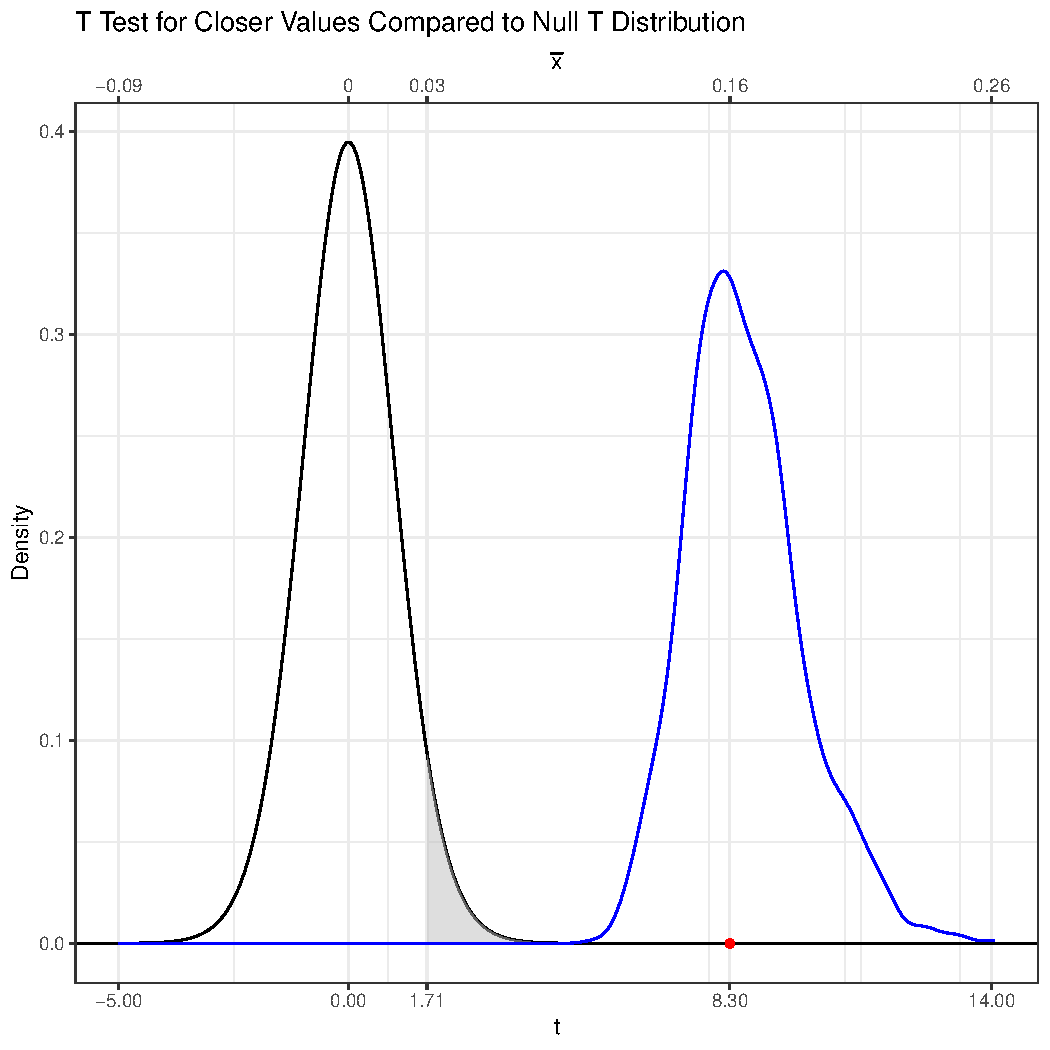
\includegraphics[width=\maxwidth]{figure/unnamed-chunk-10-1} 
\end{knitrout}
  \item Question 4, part(b).
\begin{knitrout}\scriptsize
\definecolor{shadecolor}{rgb}{0.969, 0.969, 0.969}\color{fgcolor}\begin{kframe}
\begin{alltt}
\hlcom{# b) Farther}

\hldef{mu0} \hlkwb{<-} \hlnum{0}
\hldef{x} \hlkwb{<-} \hldef{fig.2g.data}\hlopt{$}\hldef{g.Farther_vals}
\hldef{xbar} \hlkwb{<-} \hlkwd{mean}\hldef{(x)}
\hldef{s} \hlkwb{<-} \hlkwd{sd}\hldef{(x)}
\hldef{n} \hlkwb{<-} \hlkwd{length}\hldef{(x)}

\hldef{ggdat.t} \hlkwb{<-} \hlkwd{tibble}\hldef{(}\hlkwc{t}\hldef{=}\hlkwd{seq}\hldef{(}\hlopt{-}\hlnum{5}\hldef{,}\hlnum{5}\hldef{,}\hlkwc{length.out}\hldef{=}\hlnum{1000}\hldef{))|>}
  \hlkwd{mutate}\hldef{(}\hlkwc{pdf.null} \hldef{=} \hlkwd{dt}\hldef{(t,} \hlkwc{df}\hldef{=n}\hlopt{-}\hlnum{1}\hldef{))}
\hlcom{# For plotting the observed point}
\hldef{ggdat.obs} \hlkwb{<-} \hlkwd{tibble}\hldef{(}\hlkwc{t} \hldef{= t.stat.b,}
                    \hlkwc{y} \hldef{=} \hlnum{0}\hldef{)} \hlcom{# to plot on x-axis}

\hlcom{# Resampling to approximate the sampling distribution }
\hlcom{# on the data}
\hldef{R} \hlkwb{<-} \hlnum{1000}
\hldef{resamples} \hlkwb{<-} \hlkwd{tibble}\hldef{(}\hlkwc{t}\hldef{=}\hlkwd{numeric}\hldef{(R))}
\hlkwa{for}\hldef{(i} \hlkwa{in} \hlnum{1}\hlopt{:}\hldef{R)\{}
  \hldef{curr.sample} \hlkwb{<-} \hlkwd{sample}\hldef{(}\hlkwc{x}\hldef{=x,}
                        \hlkwc{size}\hldef{=n,}
                        \hlkwc{replace}\hldef{=T)}
  \hldef{resamples}\hlopt{$}\hldef{t[i]} \hlkwb{=} \hldef{(}\hlkwd{mean}\hldef{(curr.sample)}\hlopt{-}\hldef{mu0)}\hlopt{/}\hldef{(}\hlkwd{sd}\hldef{(curr.sample)}\hlopt{/}\hlkwd{sqrt}\hldef{(n))}
\hldef{\}}

\hldef{t.breaks} \hlkwb{<-} \hlkwd{c}\hldef{(}\hlopt{-}\hlnum{14}\hldef{,} \hlkwd{qt}\hldef{(}\hlnum{0.05}\hldef{,} \hlkwc{df} \hldef{= n}\hlopt{-}\hlnum{1}\hldef{),} \hlcom{# rejection region (left)}
              \hlnum{0}\hldef{,} \hlnum{5}\hldef{,}
              \hldef{t.stat.b)}                  \hlcom{# t-statistic observed}
\hldef{xbar.breaks} \hlkwb{<-} \hldef{t.breaks} \hlopt{*} \hldef{s}\hlopt{/}\hldef{(}\hlkwd{sqrt}\hldef{(n))} \hlopt{+} \hldef{mu0}

\hlcom{# Create Plot}
\hlkwd{ggplot}\hldef{()} \hlopt{+}
  \hlcom{# null distribution}
  \hlkwd{geom_line}\hldef{(}\hlkwc{data}\hldef{=ggdat.t,}
            \hlkwd{aes}\hldef{(}\hlkwc{x}\hldef{=t,} \hlkwc{y}\hldef{=pdf.null))}\hlopt{+}
  \hlkwd{geom_hline}\hldef{(}\hlkwc{yintercept}\hldef{=}\hlnum{0}\hldef{)}\hlopt{+}
  \hlcom{# rejection region}
  \hlkwd{geom_ribbon}\hldef{(}\hlkwc{data}\hldef{=}\hlkwd{subset}\hldef{(ggdat.t, t}\hlopt{<=}\hlkwd{qt}\hldef{(}\hlnum{0.05}\hldef{,} \hlkwc{df}\hldef{=n}\hlopt{-}\hlnum{1}\hldef{)),}
              \hlkwd{aes}\hldef{(}\hlkwc{x}\hldef{=t,} \hlkwc{ymin}\hldef{=}\hlnum{0}\hldef{,} \hlkwc{ymax}\hldef{=pdf.null),}
              \hlkwc{fill}\hldef{=}\hlsng{"grey"}\hldef{,} \hlkwc{alpha}\hldef{=}\hlnum{0.5}\hldef{)}\hlopt{+}
  \hlcom{# plot p-value (not visible)}
  \hlkwd{geom_ribbon}\hldef{(}\hlkwc{data}\hldef{=}\hlkwd{subset}\hldef{(ggdat.t, t}\hlopt{>=}\hldef{t.stat.b),}
              \hlkwd{aes}\hldef{(}\hlkwc{x}\hldef{=t,} \hlkwc{ymin}\hldef{=}\hlnum{0}\hldef{,} \hlkwc{ymax}\hldef{=pdf.null),}
              \hlkwc{fill}\hldef{=}\hlsng{"white"}\hldef{,} \hlkwc{alpha}\hldef{=}\hlnum{0.25}\hldef{)}\hlopt{+}
  \hlcom{# plot observation point}
  \hlkwd{geom_point}\hldef{(}\hlkwc{data}\hldef{=ggdat.obs,} \hlkwd{aes}\hldef{(}\hlkwc{x}\hldef{=t,} \hlkwc{y}\hldef{=y),} \hlkwc{color}\hldef{=}\hlsng{"red"}\hldef{)}\hlopt{+}
  \hlcom{# Resampling Distribution}
  \hlkwd{stat_density}\hldef{(}\hlkwc{data}\hldef{=resamples,}
               \hlkwd{aes}\hldef{(}\hlkwc{x}\hldef{=t),}
               \hlkwc{geom}\hldef{=}\hlsng{"line"}\hldef{,} \hlkwc{color}\hldef{=}\hlsng{"blue"}\hldef{)}\hlopt{+}
  \hlcom{# clean up aesthetics}
  \hlkwd{theme_bw}\hldef{()}\hlopt{+}
  \hlkwd{scale_x_continuous}\hldef{(}\hlsng{"t"}\hldef{,}
                     \hlkwc{breaks} \hldef{=} \hlkwd{round}\hldef{(t.breaks,}\hlnum{2}\hldef{),}
                     \hlkwc{sec.axis} \hldef{=} \hlkwd{sec_axis}\hldef{(}\hlopt{~}\hldef{.,}
                                         \hlkwc{name} \hldef{=} \hlkwd{bquote}\hldef{(}\hlkwd{bar}\hldef{(x)),}
                                         \hlkwc{breaks} \hldef{= t.breaks,}
                                         \hlkwc{labels} \hldef{=} \hlkwd{round}\hldef{(xbar.breaks,}\hlnum{2}\hldef{)))} \hlopt{+}
  \hlkwd{ylab}\hldef{(}\hlsng{"Density"}\hldef{)}\hlopt{+}
  \hlkwd{ggtitle}\hldef{(}\hlsng{"T Test for Farther Values Compared to Null T Distribution"}\hldef{)}
\end{alltt}
\end{kframe}
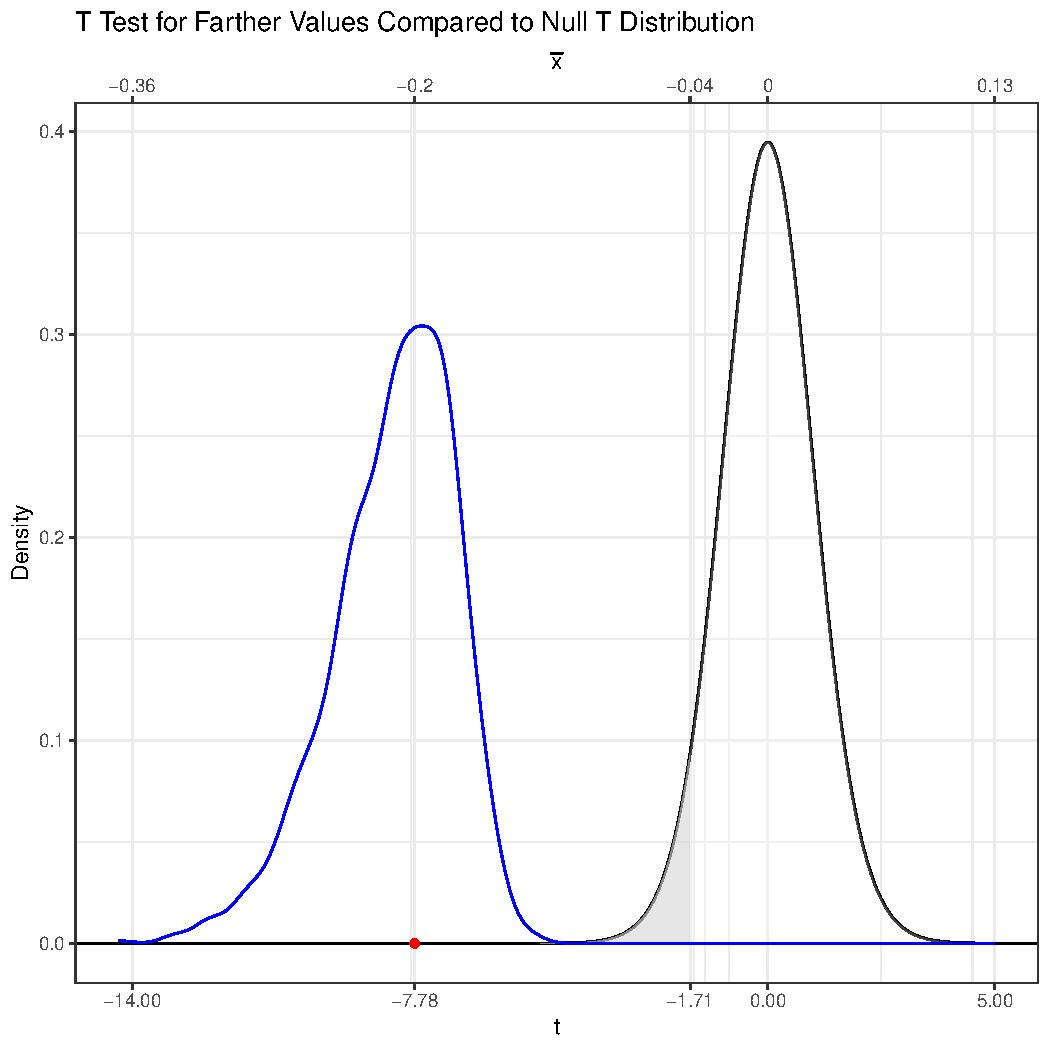
\includegraphics[width=\maxwidth]{figure/unnamed-chunk-11-1} 
\end{knitrout}
  \item Question 4, part(c).
\begin{knitrout}\scriptsize
\definecolor{shadecolor}{rgb}{0.969, 0.969, 0.969}\color{fgcolor}\begin{kframe}
\begin{alltt}
\hlcom{# c) Difference}

\hldef{mu0} \hlkwb{<-} \hlnum{0}
\hldef{x} \hlkwb{<-} \hldef{fig.2g.data}\hlopt{$}\hldef{difference}
\hldef{xbar} \hlkwb{<-} \hlkwd{mean}\hldef{(x)}
\hldef{s} \hlkwb{<-} \hlkwd{sd}\hldef{(x)}
\hldef{n} \hlkwb{<-} \hlkwd{length}\hldef{(x)}

\hldef{ggdat.t} \hlkwb{<-} \hlkwd{tibble}\hldef{(}\hlkwc{t}\hldef{=}\hlkwd{seq}\hldef{(}\hlopt{-}\hlnum{5}\hldef{,}\hlnum{5}\hldef{,}\hlkwc{length.out}\hldef{=}\hlnum{1000}\hldef{))|>}
  \hlkwd{mutate}\hldef{(}\hlkwc{pdf.null} \hldef{=} \hlkwd{dt}\hldef{(t,} \hlkwc{df}\hldef{=n}\hlopt{-}\hlnum{1}\hldef{))}
\hlcom{# For plotting the observed point}
\hldef{ggdat.obs} \hlkwb{<-} \hlkwd{tibble}\hldef{(}\hlkwc{t} \hldef{= t.stat.c,}
                    \hlkwc{y} \hldef{=} \hlnum{0}\hldef{)} \hlcom{# to plot on x-axis}

\hlcom{# Resampling to approximate the sampling distribution }
\hlcom{# on the data}
\hldef{R} \hlkwb{<-} \hlnum{1000}
\hldef{resamples} \hlkwb{<-} \hlkwd{tibble}\hldef{(}\hlkwc{t}\hldef{=}\hlkwd{numeric}\hldef{(R))}
\hlkwa{for}\hldef{(i} \hlkwa{in} \hlnum{1}\hlopt{:}\hldef{R)\{}
  \hldef{curr.sample} \hlkwb{<-} \hlkwd{sample}\hldef{(}\hlkwc{x}\hldef{=x,}
                        \hlkwc{size}\hldef{=n,}
                        \hlkwc{replace}\hldef{=T)}
  \hldef{resamples}\hlopt{$}\hldef{t[i]} \hlkwb{=} \hldef{(}\hlkwd{mean}\hldef{(curr.sample)}\hlopt{-}\hldef{mu0)}\hlopt{/}\hldef{(}\hlkwd{sd}\hldef{(curr.sample)}\hlopt{/}\hlkwd{sqrt}\hldef{(n))}
\hldef{\}}

\hldef{t.breaks} \hlkwb{<-} \hlkwd{c}\hldef{(}\hlopt{-}\hlnum{5}\hldef{,} \hlkwd{qt}\hldef{(}\hlnum{0.025}\hldef{,} \hlkwc{df} \hldef{= n}\hlopt{-}\hlnum{1}\hldef{),} \hlcom{# rejection region (left)}
              \hlnum{0}\hldef{,}
              \hlkwd{qt}\hldef{(}\hlnum{0.975}\hldef{,} \hlkwc{df} \hldef{= n}\hlopt{-}\hlnum{1}\hldef{),} \hlnum{14}\hldef{,}  \hlcom{# rejection region (right)}
              \hldef{t.stat.c)}                  \hlcom{# t-statistic observed}
\hldef{xbar.breaks} \hlkwb{<-} \hldef{t.breaks} \hlopt{*} \hldef{s}\hlopt{/}\hldef{(}\hlkwd{sqrt}\hldef{(n))} \hlopt{+} \hldef{mu0}

\hlcom{# Create Plot}
\hlkwd{ggplot}\hldef{()} \hlopt{+}
  \hlcom{# null distribution}
  \hlkwd{geom_line}\hldef{(}\hlkwc{data}\hldef{=ggdat.t,}
            \hlkwd{aes}\hldef{(}\hlkwc{x}\hldef{=t,} \hlkwc{y}\hldef{=pdf.null))}\hlopt{+}
  \hlkwd{geom_hline}\hldef{(}\hlkwc{yintercept}\hldef{=}\hlnum{0}\hldef{)}\hlopt{+}
  \hlcom{# rejection region}
  \hlkwd{geom_ribbon}\hldef{(}\hlkwc{data}\hldef{=}\hlkwd{subset}\hldef{(ggdat.t, t}\hlopt{<=}\hlkwd{qt}\hldef{(}\hlnum{0.025}\hldef{,} \hlkwc{df}\hldef{=n}\hlopt{-}\hlnum{1}\hldef{)),}
              \hlkwd{aes}\hldef{(}\hlkwc{x}\hldef{=t,} \hlkwc{ymin}\hldef{=}\hlnum{0}\hldef{,} \hlkwc{ymax}\hldef{=pdf.null),}
              \hlkwc{fill}\hldef{=}\hlsng{"grey"}\hldef{,} \hlkwc{alpha}\hldef{=}\hlnum{0.5}\hldef{)}\hlopt{+}
  \hlkwd{geom_ribbon}\hldef{(}\hlkwc{data}\hldef{=}\hlkwd{subset}\hldef{(ggdat.t, t}\hlopt{>=}\hlkwd{qt}\hldef{(}\hlnum{0.975}\hldef{,} \hlkwc{df}\hldef{=n}\hlopt{-}\hlnum{1}\hldef{)),}
              \hlkwd{aes}\hldef{(}\hlkwc{x}\hldef{=t,} \hlkwc{ymin}\hldef{=}\hlnum{0}\hldef{,} \hlkwc{ymax}\hldef{=pdf.null),}
              \hlkwc{fill}\hldef{=}\hlsng{"grey"}\hldef{,} \hlkwc{alpha}\hldef{=}\hlnum{0.5}\hldef{)}\hlopt{+}
  \hlcom{# plot p-value (not visible)}
  \hlkwd{geom_ribbon}\hldef{(}\hlkwc{data}\hldef{=}\hlkwd{subset}\hldef{(ggdat.t, t}\hlopt{>=}\hldef{t.stat.c),}
              \hlkwd{aes}\hldef{(}\hlkwc{x}\hldef{=t,} \hlkwc{ymin}\hldef{=}\hlnum{0}\hldef{,} \hlkwc{ymax}\hldef{=pdf.null),}
              \hlkwc{fill}\hldef{=}\hlsng{"white"}\hldef{,} \hlkwc{alpha}\hldef{=}\hlnum{0.25}\hldef{)}\hlopt{+}
  \hlcom{# plot observation point}
  \hlkwd{geom_point}\hldef{(}\hlkwc{data}\hldef{=ggdat.obs,} \hlkwd{aes}\hldef{(}\hlkwc{x}\hldef{=t,} \hlkwc{y}\hldef{=y),} \hlkwc{color}\hldef{=}\hlsng{"red"}\hldef{)}\hlopt{+}
  \hlcom{# Resampling Distribution}
  \hlkwd{stat_density}\hldef{(}\hlkwc{data}\hldef{=resamples,}
               \hlkwd{aes}\hldef{(}\hlkwc{x}\hldef{=t),}
               \hlkwc{geom}\hldef{=}\hlsng{"line"}\hldef{,} \hlkwc{color}\hldef{=}\hlsng{"blue"}\hldef{)}\hlopt{+}
  \hlcom{# clean up aesthetics}
  \hlkwd{theme_bw}\hldef{()}\hlopt{+}
  \hlkwd{scale_x_continuous}\hldef{(}\hlsng{"t"}\hldef{,}
                     \hlkwc{breaks} \hldef{=} \hlkwd{round}\hldef{(t.breaks,}\hlnum{2}\hldef{),}
                     \hlkwc{sec.axis} \hldef{=} \hlkwd{sec_axis}\hldef{(}\hlopt{~}\hldef{.,}
                                         \hlkwc{name} \hldef{=} \hlkwd{bquote}\hldef{(}\hlkwd{bar}\hldef{(x)),}
                                         \hlkwc{breaks} \hldef{= t.breaks,}
                                         \hlkwc{labels} \hldef{=} \hlkwd{round}\hldef{(xbar.breaks,}\hlnum{2}\hldef{)))} \hlopt{+}
  \hlkwd{ylab}\hldef{(}\hlsng{"Density"}\hldef{)}\hlopt{+}
  \hlkwd{ggtitle}\hldef{(}\hlsng{"T Test for Difference Compared to Null T Distribution"}\hldef{)}
\end{alltt}
\end{kframe}
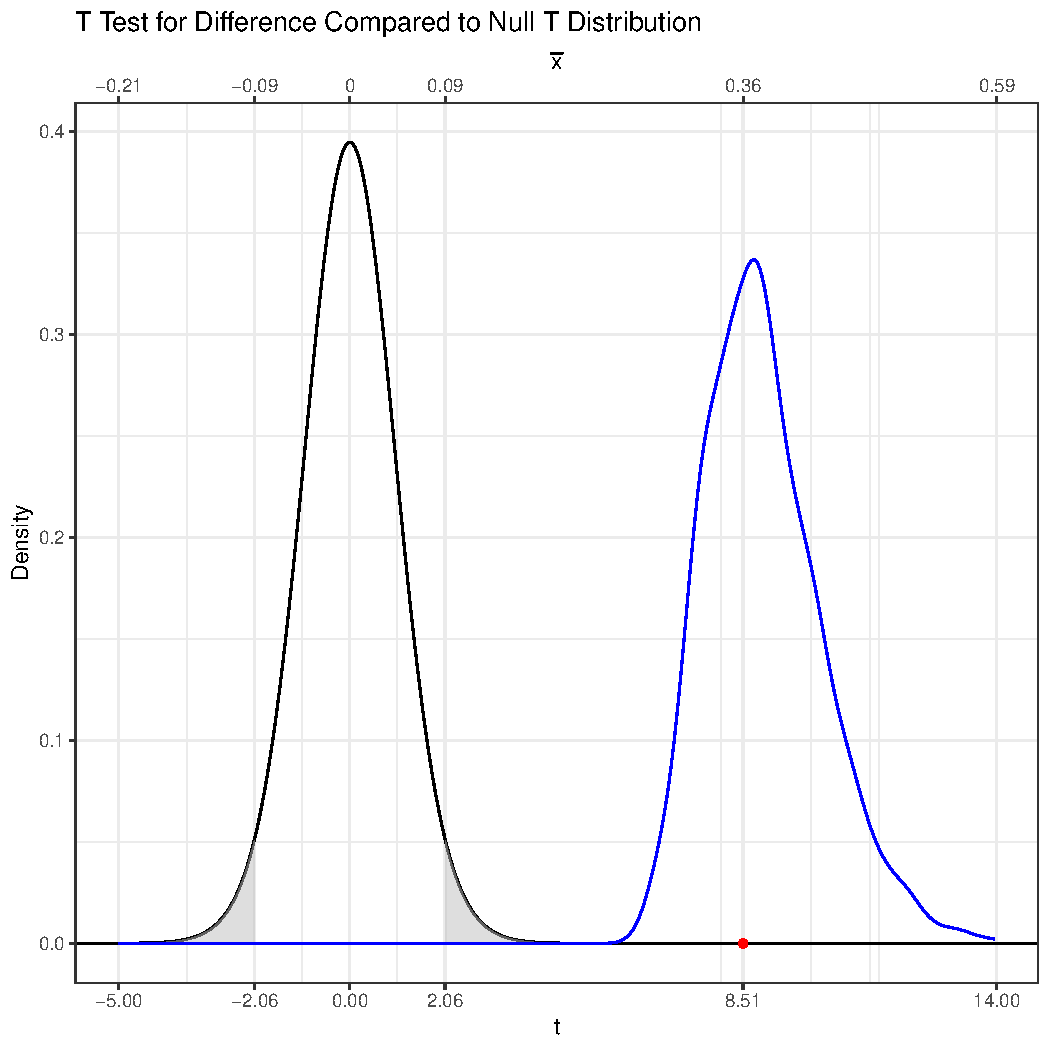
\includegraphics[width=\maxwidth]{figure/unnamed-chunk-12-1} 
\end{knitrout}

\end{enumerate}
\end{enumerate}


\bibliography{bibliography}
\end{document}
